\documentclass[12pt]{beamer}
\usepackage[polytechnique, psc, complexe, unicouleur]{persobeamer}
%nocouleur ou: unicouleur ou : bicouleur
%complexe ou : simple
%voir dans le package pour changer les couleurs
\usepackage{tikz}

\title{Projet Scientifique collectif INF02}
\subtitle{Soutenance finale}
\author{}
\date{19 mai 2015}


\begin{document}

  \addtobeamertemplate{frametitle}{}{
    \begin{tikzpicture}[remember picture,overlay]
    \node[anchor=south east,yshift=2pt] at (current page.south east) {
\includegraphics[height=0.7cm]{logohori.eps}};

    \end{tikzpicture}
   }

    \begin{frame}
      \maketitle
    \end{frame}		


    %% sommaire %%		
    \begin{frame}
      \frametitle{Sommaire}
      %\tableofcontents[pausesections]
      \tableofcontents
    \end{frame}

%%%%%%%%%%%%%%%%%%%%%%%%
\section{Rappel du projet}
%%%%%%%%%%%%%%%%%%%%%%%%%%

%%%%%%%%%%%%%%%%
\begin{frame}
 \frametitle{But du projet}
 

\end{frame}

%%%%%%%%%%%%%%%%%%%
\begin{frame}
 \frametitle{Modules}
 
 
\end{frame}


\begin{frame}
 \frametitle{Outils extérieurs et points techniques}
 
 
\end{frame}

%%je pense qu'on peut franchement réduire l'état de l'art,
%% à un bref rappel.
%ce n'est pas ce qu'ils veulent entendre à une soutenance
\section{État de l'art}

\begin{frame}
 \frametitle{Traitement du langage naturel}
 
 
\end{frame}

\begin{frame}
 \frametitle{\textit{Extractive summarization}}
 
 
\end{frame}

\begin{frame}
 \frametitle{\textit{Abstractive summarization}}
 
 
\end{frame}


\begin{frame}
 \frametitle{Génération du résumé et évaluation}
 
 
\end{frame}

%je vire copycat/bascet, on détaillera mieux
%%sur le RC lui-même

\section{Sources de données}

\subsection{Données textuelles}

\begin{frame}
 \frametitle{Données textuelles}
 
 
\end{frame}

\subsection{Données conceptuelles}

\begin{frame}
 \frametitle{Extraction de concepts}
 
 
\end{frame}

\begin{frame}
 \frametitle{WordNet}
 
 
\end{frame}

\begin{frame}
 \frametitle{Conceptnet5}
 
 
\end{frame}

\begin{frame}
 \frametitle{Freebase}
 
 
\end{frame}


%%%%%%%%%%%%%%%%%%%%%%%%%%%
\section{Réseau de concepts}
%%%%%%%%%%%%%%%%%%%%%%%%%%%
% Schrotty !

\subsection{Structure}

\begin{frame}
 \frametitle{Objectifs et utilité du réseau}
 
 \begin{itemize}
  \item Représenter des données conceptuelles ;
  \item Établir des relations sémantiques ;
  \item Fournir des informations de contexte.
 \end{itemize}
 
 Le réseau n'effectue pas la \textbf{sélection} de l'information, mais il en ajoute.
 
\end{frame}


\begin{frame}[allowframebreaks = 0.7]
 \frametitle{Structure statique du réseau}
 
\begin{block}{N\oe uds}
\begin{itemize}
 \item Étiquette : concept ;
 \item Importance conceptuelle ;
 \item Activation ;
\end{itemize}

Exemple : ["hyperactivity", "ic": 34, "a": 10].

\end{block}
 
\begin{block}{Arêtes}
 \begin{itemize}
  \item Orientées ;
  \item Proximité ;
  \item Relation.
 \end{itemize}

Exemple : ["hyperactivity", "disorder", {"r": "IsA", "w": 47}].
 
\end{block}

 
\end{frame}

%%%%%%%%%%%%%%%%%%%%%%%%%%%%%%%%%%%%%%%
\begin{frame}
 \frametitle{Propriétés dynamiques du réseau}
 
 \begin{itemize}
  \item  L'activation d'un n\oe ud se propage à ses fils ;
  \item Les n\oe uds se désactivent naturellement.
 \end{itemize}
 
 Exemple 1 : en partant de "wayne rooney" et  "manchester united f.c.".
 
 Exemple 2 : en considérant les n\oe uds fortement activés (plus de 10\%).
 
 \note{Sur ce premier exemple, on ne montre pas le degré d'activation de chaque noeud, c'est juste pour voir la propagation. Sur le deuxième on s'intéresse déjà plus à la pertinence.}
 
\end{frame}


%%%%%%%%%%%%%%%%%%%%%%%%%%%%%%%
\begin{frame}
  \frametitle{Exemple 1}
  
  %\iffalse
  
  \begin{block}{Nombre de n\oe uds activés}
   \begin{overprint}
\onslide<1> Étape 0 : 2
\onslide<2> Étape 1 : 6
\onslide<3> Étape 2 : 67
\onslide<4> Étape 3 : 51
\onslide<5> Étape 4 : 59
\onslide<6> Étape 5 : 133
\end{overprint}
  \end{block}

  
  \begin{overlayarea}{8cm}{8cm}
   \only<1>{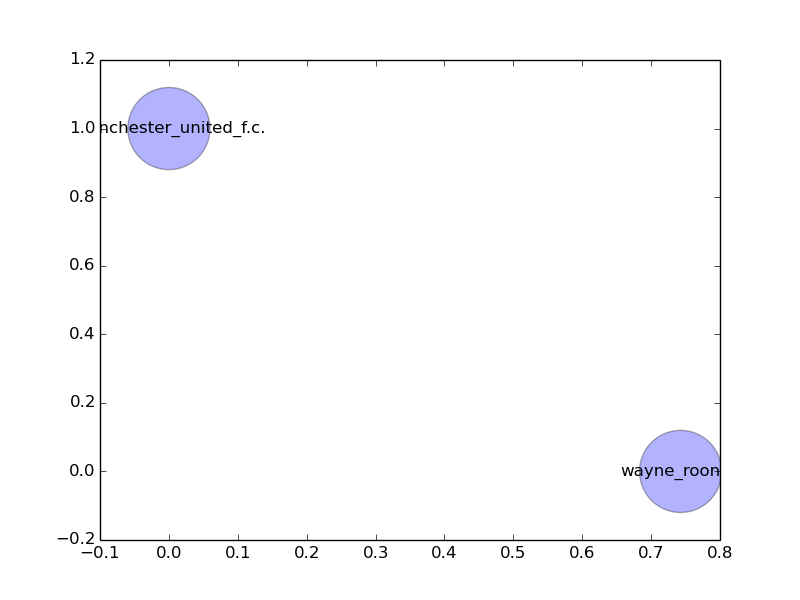
\includegraphics[height=7cm]{examples/touslesnoeuds/0.png}}
   \only<2>{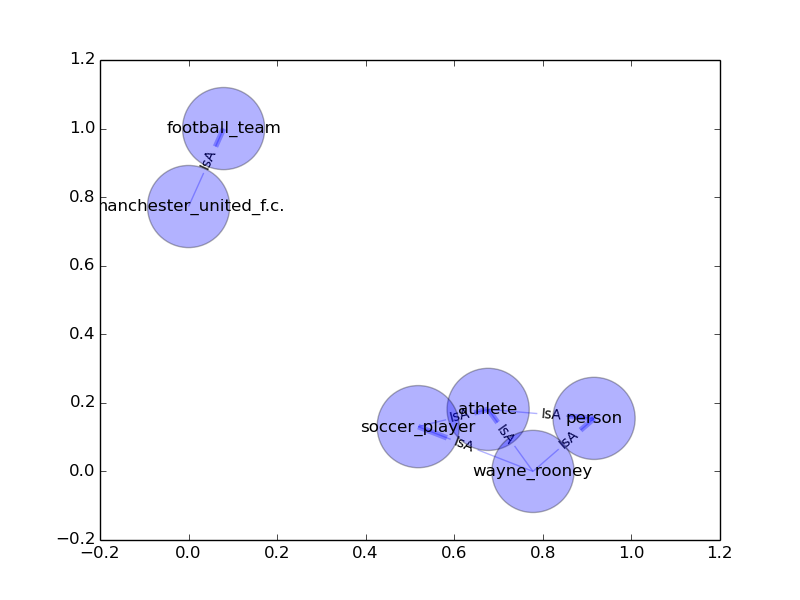
\includegraphics[height=7cm]{examples/touslesnoeuds/1.png}}
   \only<3>{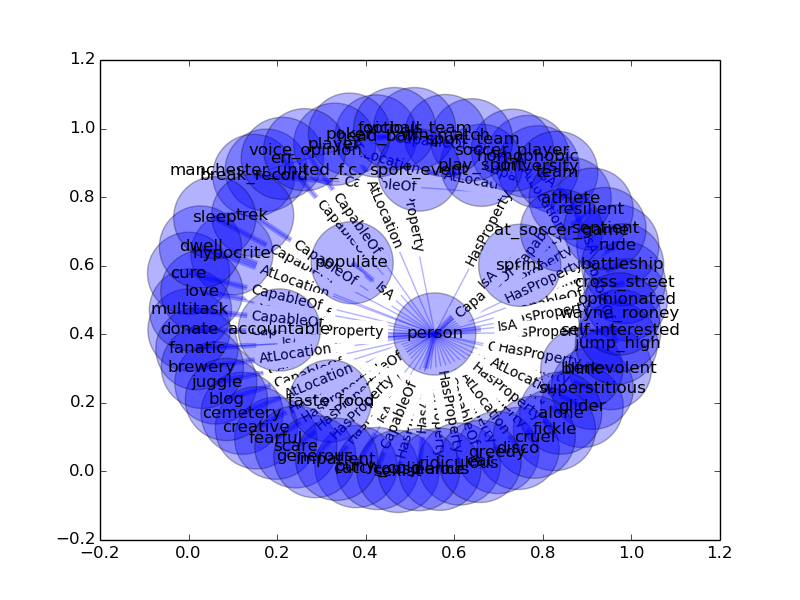
\includegraphics[height=7cm]{examples/touslesnoeuds/2.png}}
   \only<4>{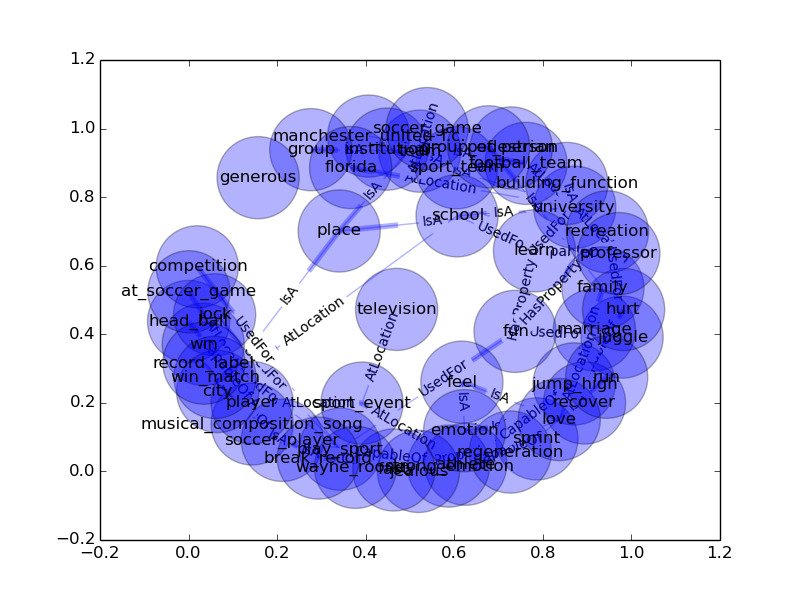
\includegraphics[height=7cm]{examples/touslesnoeuds/3.png}}
   \only<5>{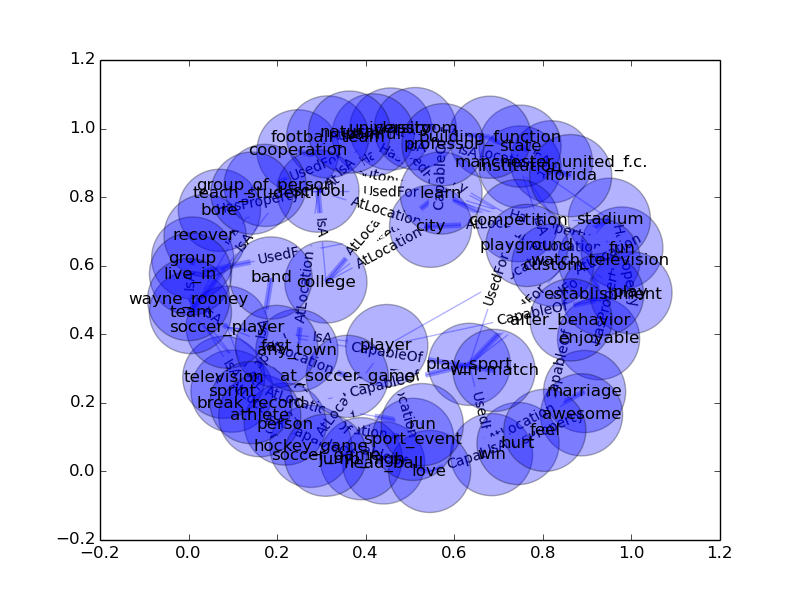
\includegraphics[height=7cm]{examples/touslesnoeuds/4.png}}
   \only<6>{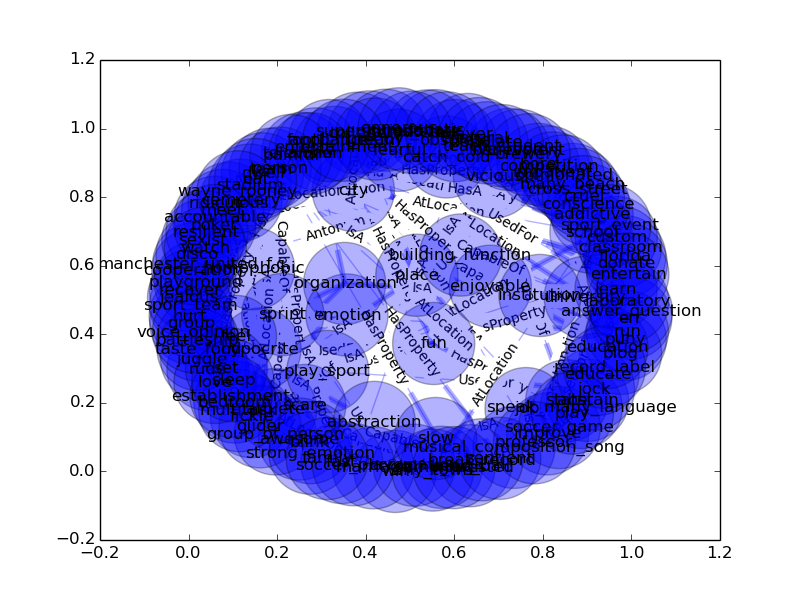
\includegraphics[height=7cm]{examples/touslesnoeuds/5.png}}
   \only<7>{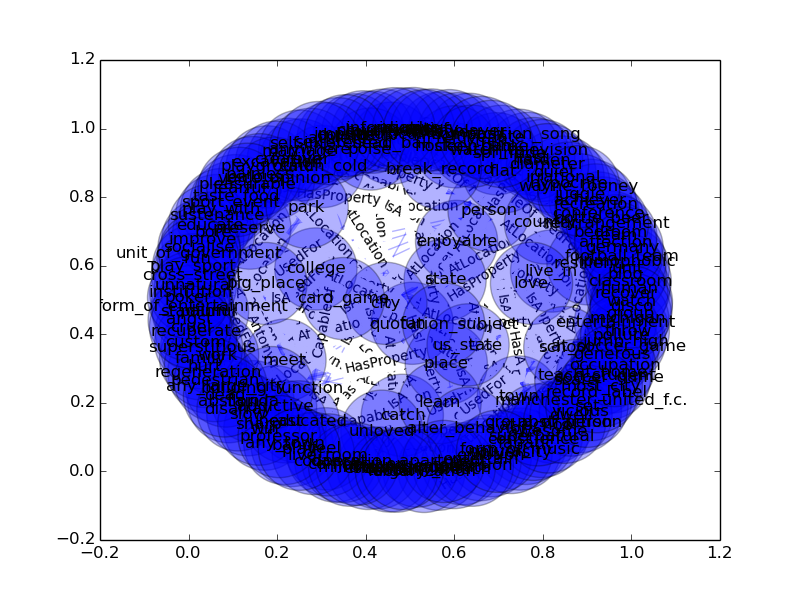
\includegraphics[height=7cm]{examples/touslesnoeuds/6.png}}
  \end{overlayarea}

 % \fi

\end{frame}


\begin{frame}
  \frametitle{Exemple 2}
  
  %\iffalse
  
  \begin{block}{Nombre de n\oe uds activés}
   \begin{overprint}
\onslide<1> Étape 0 : 2
\onslide<2> Étape 1 : 3
\onslide<3> Étape 2 : 4
\onslide<4> Étape 3 : 4
\onslide<5> Étape 4 : 5
\onslide<6> Étape 5 : 9
\onslide<7> Étape 6 : 16
\onslide<8> Étape 7 : 22
\onslide<9> Étape 8 : 34
\onslide<10> Étape 9 : 54
\end{overprint}
  \end{block}

  
  \begin{overlayarea}{8cm}{8cm}
   \only<1>{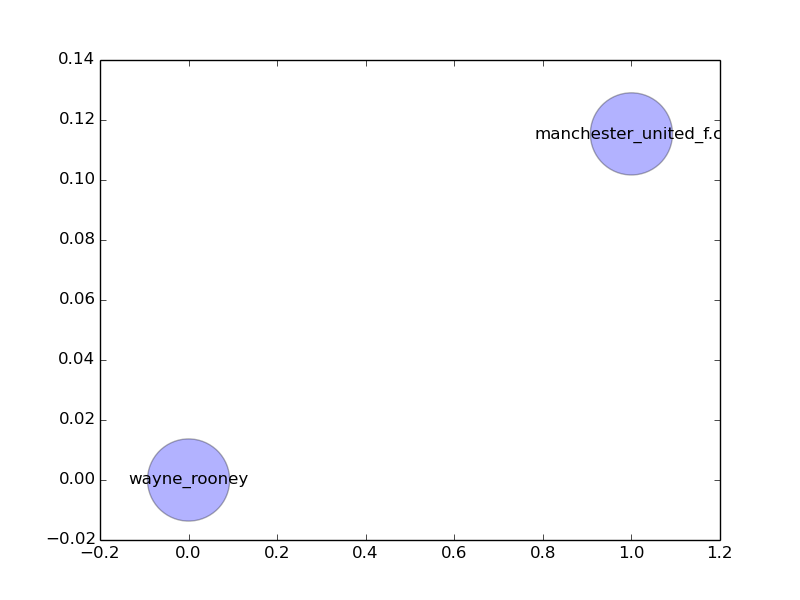
\includegraphics[height=7cm]{examples/noeudsbienactives/0.png}}
   \only<2>{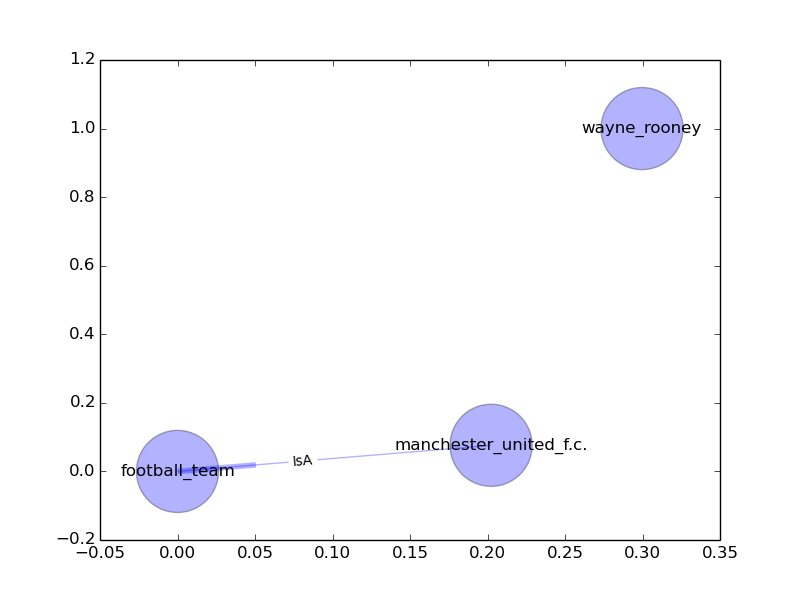
\includegraphics[height=7cm]{examples/noeudsbienactives/1.png}}
   \only<3>{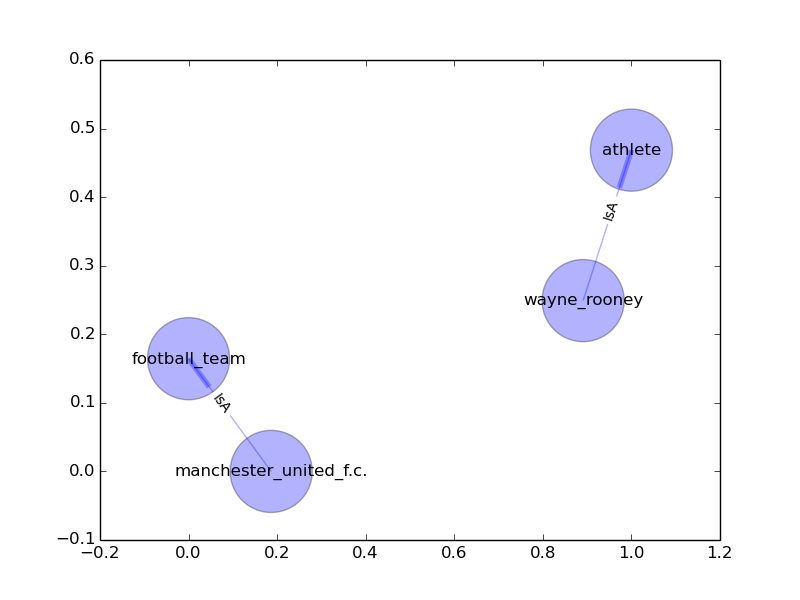
\includegraphics[height=7cm]{examples/noeudsbienactives/2.png}}
   \only<4>{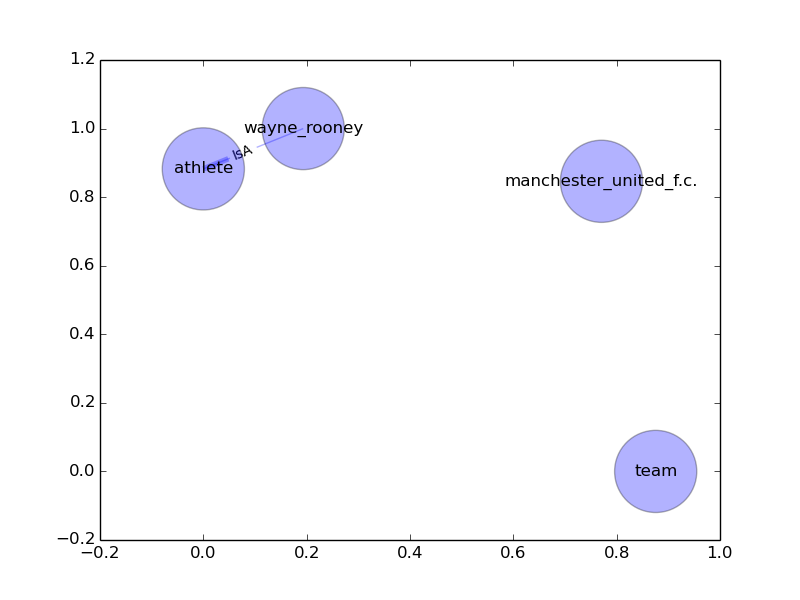
\includegraphics[height=7cm]{examples/noeudsbienactives/3.png}}
   \only<5>{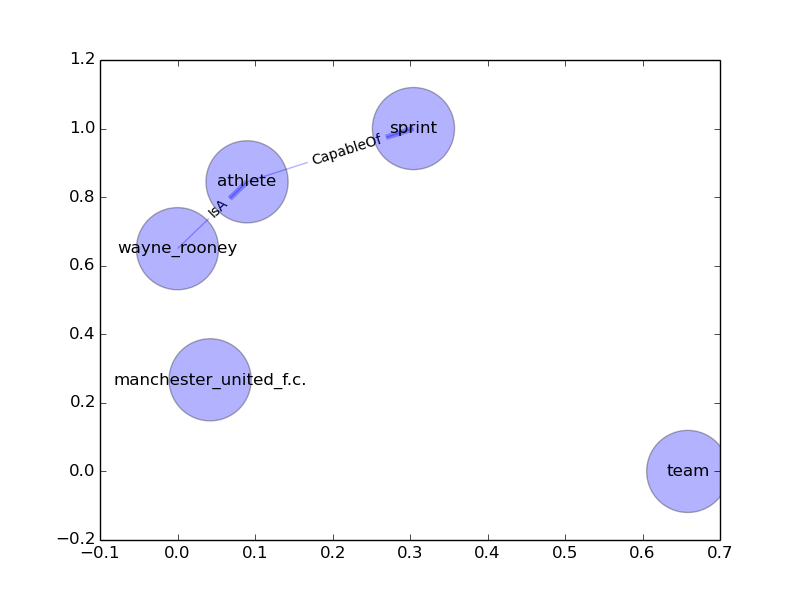
\includegraphics[height=7cm]{examples/noeudsbienactives/4.png}}
   \only<6>{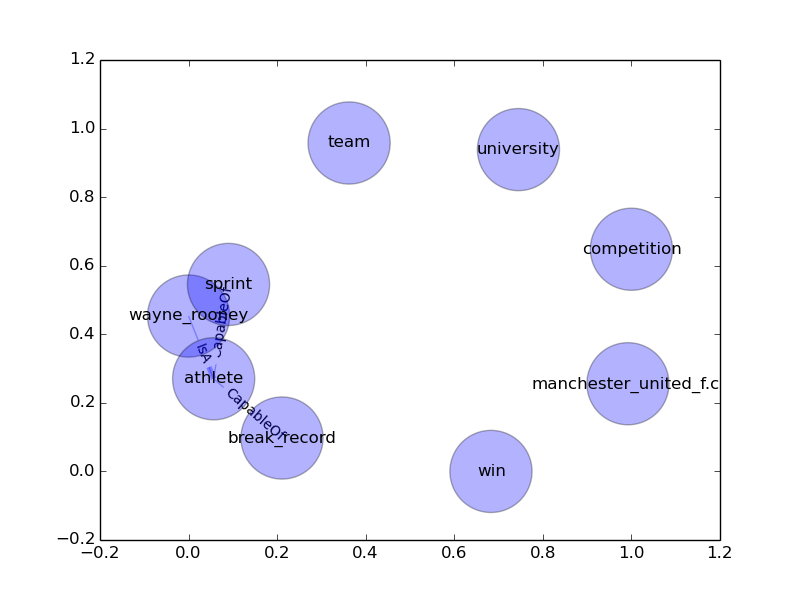
\includegraphics[height=7cm]{examples/noeudsbienactives/5.png}}
   \only<7>{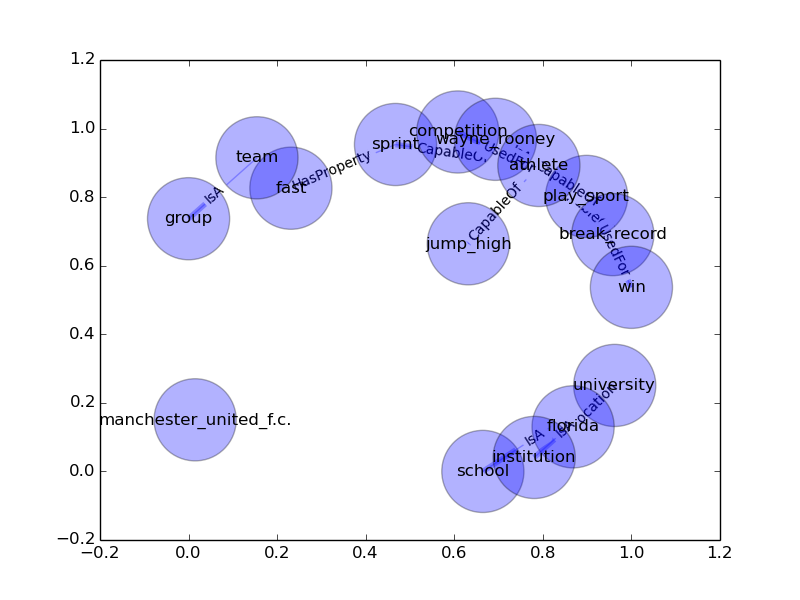
\includegraphics[height=7cm]{examples/noeudsbienactives/6.png}}
   \only<8>{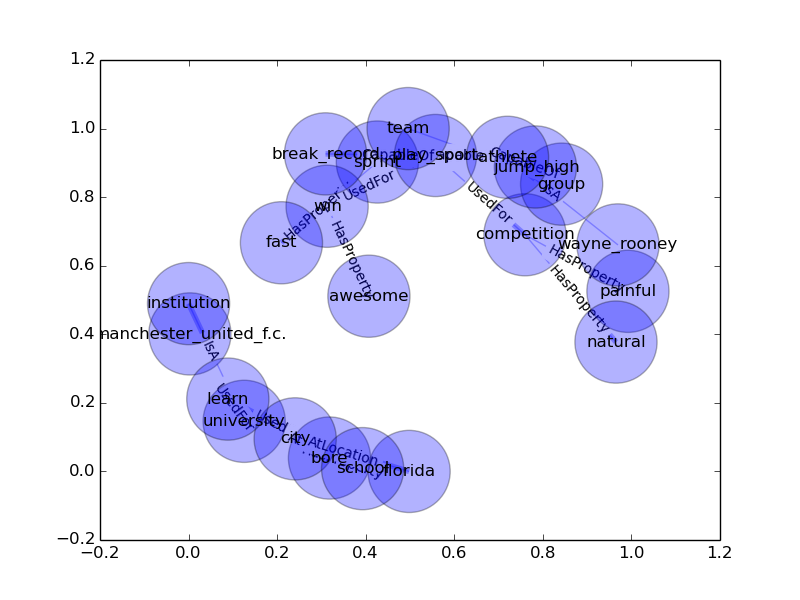
\includegraphics[height=7cm]{examples/noeudsbienactives/7.png}}
   \only<9>{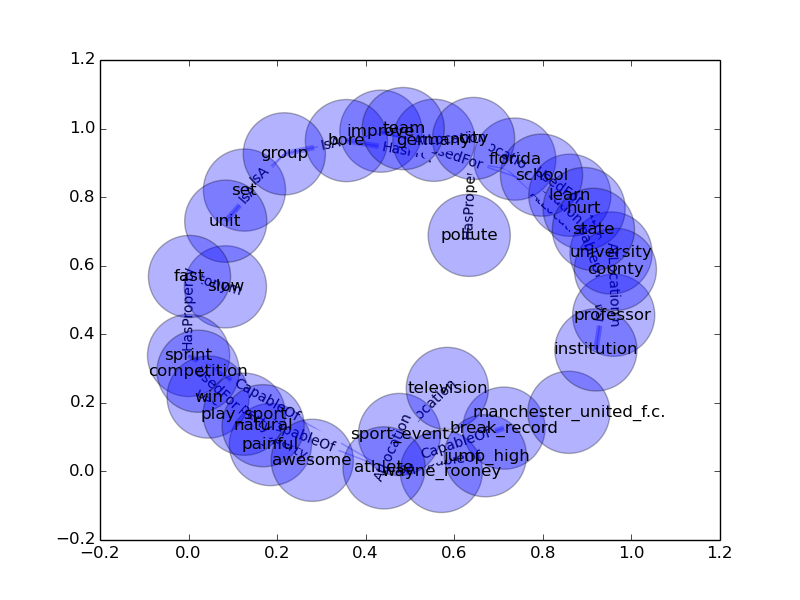
\includegraphics[height=7cm]{examples/noeudsbienactives/8.png}}
   \only<10>{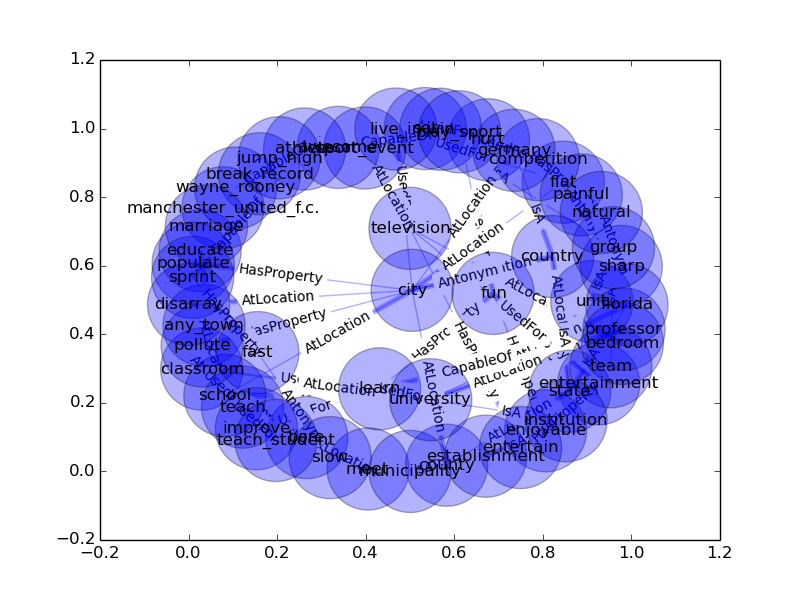
\includegraphics[height=7cm]{examples/noeudsbienactives/9.png}}
  \end{overlayarea}

 % \fi
  
\end{frame}

%%%%%%%%%%%%%%%%%%%%%%%%%%%%%%%
\begin{frame}[allowframebreaks = 0.7]
 \frametitle{Détails}
 
 \begin{itemize}
  \item Les concepts "font penser" à d'autres concepts : contexte ;
  \item Certains concepts sont oubliés : sélection.
 \end{itemize}

 On ne cherche pas un état d'équilibre. Il faut tirer parti de ces deux propriétés en réglant le nombre d'étapes.
 
 \begin{block}{Comment désactiver ?}
 \begin{itemize}
  \item En fonction de l'importance conceptuelle ;
  \item En fonction du nombre de liens.
  \end{itemize}
 \end{block}

 Exemple 3 :  N\oe uds bien activés, sans tenir compte du nombre de liens.
 
 \note{!!!! Pour l'importance conceptuelle, on verra plus tard avec les méthodes statistiques. Même exemple que le deuxième, mais avec cette fois un facteur log égal à 1, donc aucune dépendance avec le nombre de liens.}
 
\end{frame}


%%%%%%%%%%%%%%%%%%%%%%%%%%%%%%%%%
\begin{frame}
\frametitle{Exemple 3}

%\iffalse

  \begin{block}{Nombre de n\oe uds activés}
   \begin{overprint}
\onslide<1> Étape 0 : 2
Étape 1 : 5
Étape 2 : 14
Étape 3 : 26
Étape 4 : 51
Étape 5 : 114
Étape 6 : 209
Étape 7 : 334
Étape 8 : 535
Étape 9 : 765
Étape 10 : 1060
Étape 11 : 1363
Étape 12 : 1644

\end{overprint}
  \end{block}

  
  \begin{overlayarea}{8cm}{8cm}
   \only<1>{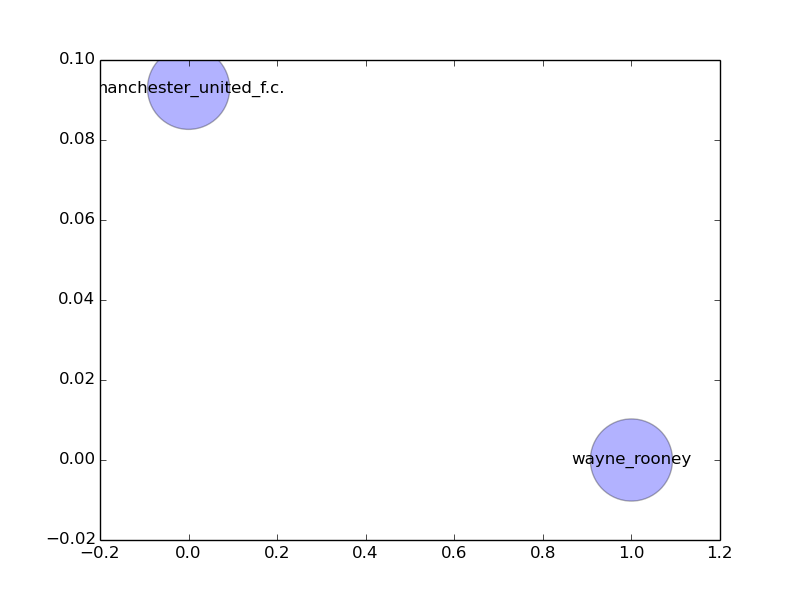
\includegraphics[height=7cm]{examples/facteurlogun/0.png}}
   \only<2>{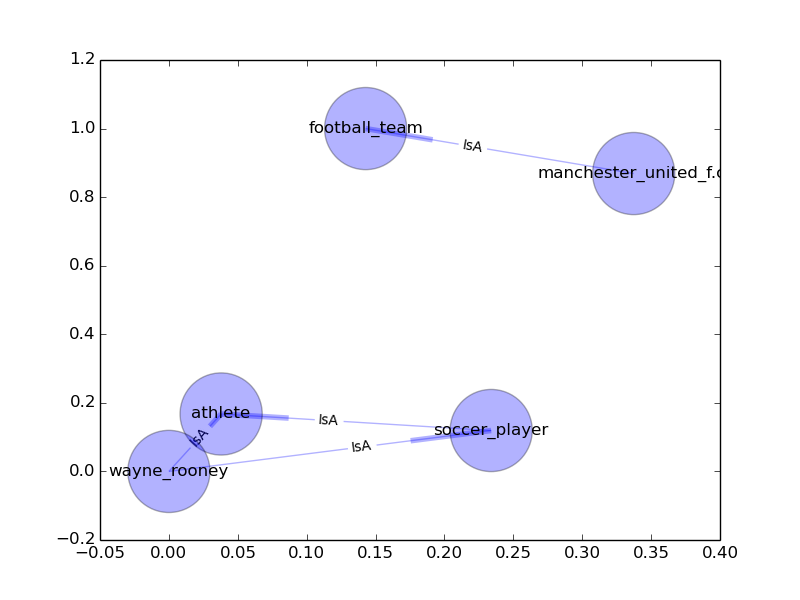
\includegraphics[height=7cm]{examples/facteurlogun/1.png}}
   \only<3>{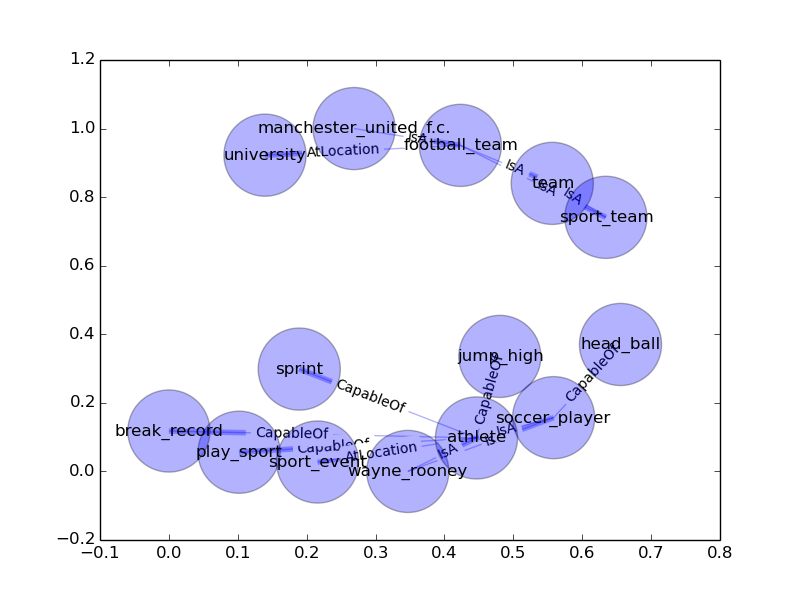
\includegraphics[height=7cm]{examples/facteurlogun/2.png}}

  \end{overlayarea}

 % \fi
  

\end{frame}


\subsection{Construction}

\begin{frame}
 \frametitle{Construction du réseau}
 
 
\end{frame}

\begin{frame}[fragile]
 \frametitle{Exemple obtenu}
 
 \begin{block}{Meilleurs en liens sortants}
 \begin{verbatim}
 human : 41
water : 44
person : 50
someone : 161
something : 192 
\end{verbatim}
 \end{block}

 \begin{block}{Meilleurs en liens entrants}
 \begin{verbatim}
  soccer_player : 1931
soccer_midfielder : 1575
athlete : 2182
person : 3469
Et bien d'autres... (organisation, country...)
\end{verbatim}
 \end{block}

\end{frame}


%%optionnel, et même beaucoup trop chiant
\begin{frame}
 \frametitle{Choix de programmation}
 
 
\end{frame}


\section{TF-IDF et méthodes statistiques}

\subsection{TF-IDF pour le résumé automatique}

\begin{frame}
 \frametitle{Définition de l'indice TF-IDF}
 
 
\end{frame}

\begin{frame}
 \frametitle{Utilisation de TF-IDF}
 
 
\end{frame}

\subsection{TF-IDF pour l'importance conceptuelle}

\begin{frame}
 \frametitle{}
 
 
\end{frame}


\section{Traitement préalable des données}

\subsection{Analyse syntaxique}

\begin{frame}
 \frametitle{Grammaires}
 
 
\end{frame}

\begin{frame}
 \frametitle{État du texte en fin d'analyse}
 
 
\end{frame}

\subsection{Résolution de pronoms}

\begin{frame}[allowframebreaks = 0.7]
 \frametitle{Résolution de pronoms}
 
 
\end{frame}

\section{Traitement du réseau}

\subsection{Workspace}

\begin{frame}
 \frametitle{Workspace}
 
 
\end{frame}

\begin{frame}
 \frametitle{}
 
 
\end{frame}

\subsection{Algorithme final}

\begin{frame}
 \frametitle{Algorithme final}
 
 
\end{frame}

\begin{frame}
 \frametitle{Exemples}
 
 
\end{frame}

\section{Conclusion}

\begin{frame}
 \frametitle{Conclusion}
 
C'était vraiment trop mythe comme PSC.
 
\end{frame}

\end{document}
